\section{Sobre Nuestra Empresa}

  \textbf{Wallpa Wawqi} es un ficticio restaurante tradicional peruano que representa el común de los negocios de comida en Perú, desde pequeños locales hasta cadenas de restaurantes. El nombre "Wallpa Wawqi" se inspira en la cultura peruana, con "Wallpa" que significa "gallina" en quechua, y "Wawqi" que significa "hermano" lo que es un guiño a la cadena de restaurantes de comida rápida "Pollos Hermanos". Como es usual en este tipo de negocios, la gestión eficaz de los datos relacionados con clientes, personal, productos y operaciones de compra y venta es crucial para la rentabilidad y el éxito del restaurante.

  Dentro del flujo de operaciones de Wallpa Wawqi, intervienen cuatro actores principales: el administrador, el cliente, el personal de servicio y los proveedores. El administrador es responsable de la gestión general del restaurante, incluyendo la supervisión del personal, la gestión de inventarios y la toma de decisiones estratégicas. El cliente es el consumidor final que realiza pedidos y consume los productos ofrecidos por el restaurante. El personal de servicio se encarga de atender a los clientes, tomar pedidos y asegurar una experiencia satisfactoria. Finalmente, los proveedores son los encargados de suministrar los ingredientes y productos necesarios para el funcionamiento del restaurante.

  La intereacción entre estos actores es lo que da vida al modelo de negocio de Wallpa Wawqi, y es precisamente esta dinámica la que se busca gestionar eficientemente a través del sistema de gestión de productos y servicios que se desarrollará en este proyecto. La correcta administración de los datos relacionados con cada uno de estos actores permitirá optimizar las operaciones del restaurante, mejorar la experiencia del cliente y aumentar la rentabilidad del negocio.

  \subsection{Logo de la Empresa}

    El logo de Wallpa Wawqi representa la identidad visual de nuestro restaurante, combinando elementos de la cultura peruana con un diseño moderno y accesible. La imagen que se presenta a continuación muestra el logotipo oficial:

    \begin{figure}[h]
      \centering
      
\includegraphics[width=0.4\textwidth]{./assets/logo_wallpa.png}
      \caption{Logo oficial de Wallpa Wawqi}
      \label{fig:logo_empresa}
    \end{figure}

    El diseño del logo incorpora simbolismo peruana a través de motivos tradicionales, reflejando el compromiso de la empresa con sus raíces culturales. Este fue realizado con ayuda de motores de inteligencia artificial generadoras de imágenes.

    \newpage

    \subsection{Paleta de Colores}

        La paleta de colores de Wallpa Wawqi está compuesta por tonos cálidos y apetitosos inspirados en el pollo a la brasa, el fuego y la gastronomía peruana. Estos colores buscan transmitir calidez, cercanía y una experiencia culinaria auténtica. Los colores principales incluyen:

        \begin{itemize}
            \item \textbf{Naranja Intenso} (\#FF5A00): Representa la energía, el dinamismo y la identidad principal de la marca. Se utiliza en botones, llamados a la acción y elementos destacados, evocando el calor del horno y la pasión culinaria.

            \item \textbf{Naranja Oscuro} (\#D96A1A): Simboliza el sabor y el carácter tradicional del restaurante, inspirado en los tonos dorados del pollo a la brasa y los ingredientes tostados.

            \item \textbf{Amarillo Dorado} (\#F4C542): Evoca el dorado característico del pollo a la brasa, transmitiendo calidez, apetito y tradición gastronómica peruana.

            \item \textbf{Blanco Suave} (\#F8F8F8): Aporta limpieza, equilibrio visual y claridad en la presentación del contenido, mejorando la legibilidad y organización de la interfaz.

            \item \textbf{Gris Oscuro} (\#333333): Utilizado para textos y elementos de navegación, aporta elegancia y contraste, favoreciendo una lectura clara y moderna.

            \item \textbf{Negro Profundo} (\#1A1A1A): Presente en fondos e imágenes destacadas, refuerza el contraste visual y transmite sofisticación y fuerza visual.
            
            \item \textbf{Rojo vino} (\#8B0000): Simboliza la pasión y el entusiasmo, inspirado en los tonos intensos del vino tinto y los ingredientes picantes.

        \end{itemize}

        \begin{figure}[h]
          \centering
          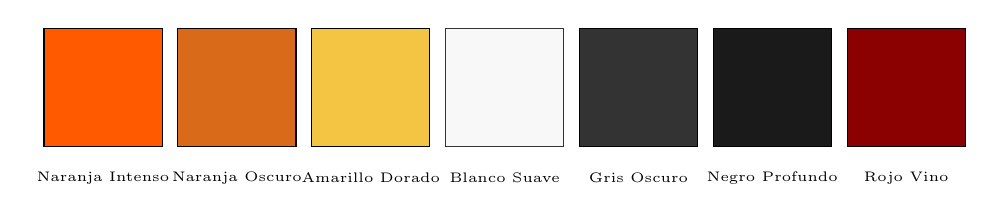
\begin{tikzpicture}
            \definecolor{naranjaIntensо}{HTML}{FF5A00}
            \definecolor{naranjaOscuro}{HTML}{D96A1A}
            \definecolor{amarilloDorado}{HTML}{F4C542}
            \definecolor{blancoSuave}{HTML}{F8F8F8}
            \definecolor{grisOscuro}{HTML}{333333}
            \definecolor{negroP}{HTML}{1A1A1A}
            \definecolor{rojoVino}{HTML}{8B0000}
            
            \draw[fill=naranjaIntensо] (0,0) rectangle (1.5,1.5);
            \draw[fill=naranjaOscuro] (1.7,0) rectangle (3.2,1.5);
            \draw[fill=amarilloDorado] (3.4,0) rectangle (4.9,1.5);
            \draw[fill=blancoSuave, draw=grisOscuro] (5.1,0) rectangle (6.6,1.5);
            \draw[fill=grisOscuro] (6.8,0) rectangle (8.3,1.5);
            \draw[fill=negroP] (8.5,0) rectangle (10,1.5);
            \draw[fill=rojoVino] (10.2,0) rectangle (11.7,1.5);
            
            \node at (0.75,-0.4) {\tiny Naranja Intenso};
            \node at (2.45,-0.4) {\tiny Naranja Oscuro};
            \node at (4.15,-0.4) {\tiny Amarillo Dorado};
            \node at (5.85,-0.4) {\tiny Blanco Suave};
            \node at (7.55,-0.4) {\tiny Gris Oscuro};
            \node at (9.25,-0.4) {\tiny Negro Profundo};
            \node at (10.95,-0.4) {\tiny Rojo Vino};
          \end{tikzpicture}
          \caption{Paleta de colores oficial de Wallpa Wawqi}
          \label{fig:paleta_colores}
            \end{figure}

        Esta paleta de colores refuerza la identidad visual de Wallpa Wawqi al transmitir sensaciones de calidez, sabor y tradición. Asimismo, contribuye a generar una experiencia visual atractiva y coherente con la temática gastronómica del restaurante, incentivando el apetito y la confianza de los clientes.
        